\lstnewenvironment{Code}[1][]{\lstset{basicstyle=\small\ttfamily, columns=fullflexible,framexrightmargin=+.1\textwidth, keywordstyle=\color{red}\bfseries, commentstyle=\color{blue},language=C++, basicstyle=\small, numbers=left, numberstyle=\tiny, stepnumber=1, numbersep=5pt, frame=shadowbox, #1}}{}

%\chapter{Descrizione Implementazione}
\section{Descrizione Implementazione}
\label{chap:Code}

In questo capitolo verranno descritte la struttura di base e le funzioni principali del codice sviluppato.
Per l'implementazione del codice si è utilizzato il solver \href{http://www.freefem.org/}\texttt{FreeFem$++$}\footnote{http://www.freefem.org/} ed il relativo linguaggio di programazione. Durante tutte le fasi di sviluppo del codice è stata utilizzata la piattaforma di hosting web \href{https://github.com/}{\texttt{GitHub}}\footnote{https://github.com/}. Questo ha sia reso più fluida la collaborazione fra gli autori che garantito un maggiore controllo sull'avanzamento del codice.

\subsection{Strumenti di sviluppo}
\subsubsection{\texttt{FreeFem$++$}}
\href{http://www.freefem.org/}\texttt{FreeFem$++$} è un software per la risoluzione di equazioni alle derivate parziali che ha un proprio linguaggio di scripting basato sul C$++$. Gli script permettono di risolvere sistemi non lineari di più variabili in un dominio 2D o 3D.
\texttt{FreeFem$++$} è un software libero, disponibile per i sistemi operativi \textit{Linux}, \textit{Solaris}, \textit{OS X} and \textit{MS Windows}.

\subsubsection{\texttt{GitHub}}
{\texttt{Git}} è un sistema di controllo versione utilizzabile direttamente da linea di comando, molto diffuso e utile per tenere traccia delle varie fasi di sviluppo del codice. \texttt{GitHub} gestisce in modo adeguato i contributi al codice provenienti da agenti esterni e permette la condivisione del codice.\\
Il codice del progetto è reperibile su \texttt{GitHub} ed è possibile scaricarlo e collabolare allo sviluppo clonando il codice dalla repository  \href{https://github.com/}{\texttt{GitHub}}:\\
\begin{center}
\texttt{ git clone https://github.com/ClaB90/Progetto\_ANEDP}
\end{center}
Nella cartella principale è contenuto anche un file \texttt{.gitignore}, in cui sono specificate le estensioni dei files e le sottocartelle che non devono essere visionati in una repository \texttt{GitHub}. In particolare non si è interessati ai files temporanei che vengono eventualmente generati dagli editor.

\subsection{Implementazione}
In questo lavoro sia l'algoritmo \ref{PuntoFisso} di punto fisso che l'algoritmo \ref{DN} di Newton  sono stati implementati per la soluzione del problema parabolico di controllo ottimo \eqref{eq:200} descritto nei capitoli precedenti.
Il corpo del programma è costituito dal file \textbf{main.edp} che permette di risolve il problema \ref{Pk} con uno dei due algoritmi su una o più griglie temporali. Il processo di raffinamento temporale considera griglie, della tipologia introdotta nella sezione \ref{chap:Discontinuos}, uniformi tali che il numero di nodi Nk al livello l di infittimento sia:
\begin{equation}
Nk = ( 2^l + 1 )
\label{Nk}
\end{equation}
I valori della soluzione approssimata $u_k$ del problema di controllo vengono salvati per ogni livello di raffinamento in dei file di testo esterni per poter esser confrontati graficamente coi valori della soluzione esatta, nei casi in cui quest'ultima sia nota.
\par
L'errore fra la soluzione esatta e la soluzione approssimata per le funzioni di stato, aggiunta e controllo viene calcolato e salvato in un file di testo ad ogni livello. Questo permette il calcolo dell'ordine di convergenza per i diversi errori.
\par
Gli altri file principali sono i seguenti:
\begin{itemize}
\item[-] \texttt{controlparameters.edp}: contiene i parametri che definiscono il problema di controllo;
\item[-] \texttt{controlfunction.edp}: contiene le funzioni per l'algoritmo \ref{PuntoFisso} di punto fisso e per semi Newton \ref{DN};
\item[-] \texttt{UabSet.edp}: contiene i parametri limite dell'insieme $U_{ad}$ e le funzioni di proiezione per uno scalare e per un vettore sullo spazio $U_{ad}$;
\item[-] \texttt{funzioni.edp} contiene le funzioni che caratterizzano l'operatore B, la funzione yd e la forzante del problema di stato $g_0$, che verrà definita nella sezione \ref{chap:Results};
\item[-] \texttt{soluzioniEsatte.edp}: definisce le funzioni per le soluzioni esatte del problema di stato y, del problema aggiunto p e per la variabile di controllo u;
\item[-] \texttt{mesh.edp}: contine la definizione del dominio, la mesh ed il paramentro N di discretizazione spaziale;
\item[-] \texttt{state.edp}: in questo file viene definito il problema di stato. In particolare vengono introdotti lo spazio degli elementi finiti, la soluzione y0 all'istante iniziale, la definizione delle matrici di Stiffness e la funzione per la risoluzione del problema di stato;
\item[-] \texttt{adjoint.edp}: in questo file viene definito il problema aggiunto. Anche in questo caso vengono introdotti lo spazio degli elementi finiti, la soluzione pT all'istante finale, la definizione delle matrici di Stiffness e la funzione per la risoluzione del problema di aggiunto; 
\item[-] \texttt{normeeprodotti.edp}: contiene tutte le funzioni implementate per il calcolo delle norme e dei prodotti scalari; 
\item[-] \texttt{funzioniErrore.edp} e \texttt{funzioniErroreAdj.edp}: contengono le funzioni per il calcolo dell'errore delle variabili y,p e u;
\item[-] \texttt{funzioniCG.edp}: contiene le funzioni necessarie per l'algoritmo del gradiente coniugato \ref{CG}; 
\item[-] \texttt{saveme.edp} e \texttt{saveerr.edp}: descrivono le funzioni per salvare i valori della soluzione approsimata di controllo e dell'aggiunto e degli errori al termine dell'algoritmo per una data griglia temporale. Inoltre contiene la funzione per il calcolo dell'ordine di convergenza dell'errore in tempo;
\end{itemize}
Per il calcolo di ogni norma e prodotto scalare il metodo numerico di integrazione in tempo utilizzato è il metodo di Cavalieri Simpson. \MakeUppercase{è} stata fatta questa scelta poichè questa formula di Newton-Cotes ha un errore di quadratura sufficientemente basso da non influenzare l'analisi degli errori oggetto di studio.
\par
Per i problemi parabolici di controllo ottimo è necessario salvare matrici molto grandi contenenti le soluzioni del problema di stato e del problema aggiunto ad ogni istante temporale considerato. Questa richesta può portare a problemi di insufficiente memoria RAM durante l'esecuzione del programma. Tuttavia in questo lavoro non sono stati riscontrati problemi di questo tipo, e per una maggiore velocità di calcolo le soluzioni sono state tenute in memoria.
\subsubsection{Calcolo dell'errore}
Per il calcolo dell'errore della soluzione approssimata $u_k$ del problema di contollo particolare attenzione è stata posta sulla griglia di integrazione. La soluzione del problema aggiunto $p_k$ è una funzione continua lineare a tratti nel tempo i cui punti di non derivabilità coincidono con i nodi della griglia. La soluzione $u_k$, equazione \eqref{cnott}, è ancora una funzione funzione continua lineare a tratti nel tempo, ma l'operazione di proiezione $P_{U_{ab}}$ non garantisce che i nodi della griglia temporale utilizzata corrispondano a i punti di non derivabilità della funzione stessa, come mostrato in Figura \ref{fig:griglie}.
\begin{figure}
\centering
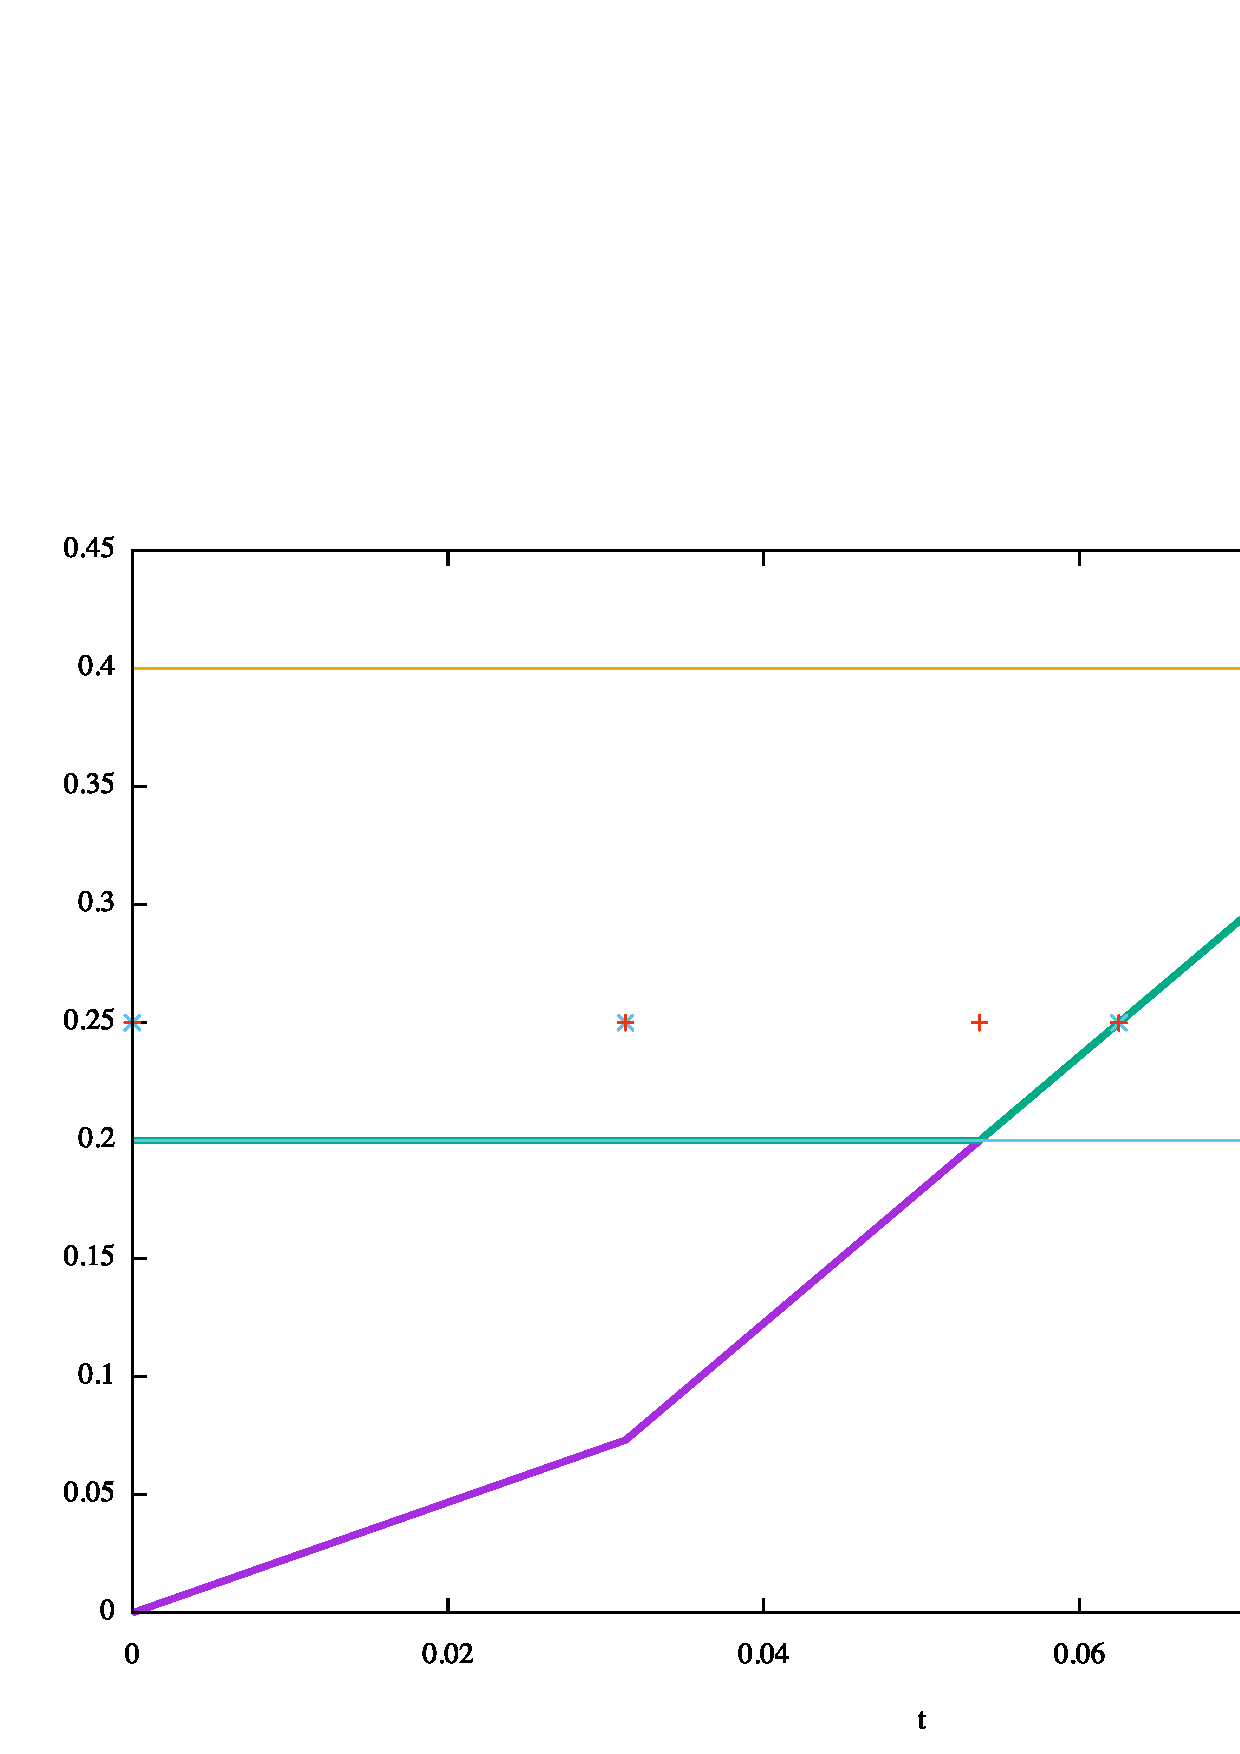
\includegraphics[scale=0.45]{img/cap5/griglie}
\caption{Esempio di differenza fra la griglia per la soluzione $u_k$ e la soluzione di $p_k$}
\label{fig:griglie}
\end{figure}
La funzione:
\begin{Code}[caption={Funzione \texttt{controlErrL2}}]
func real controlErrL2(real[int] &controlsol)
\end{Code}
Prende in ingresso la soluzione approssimata $u_k$ e calcola la norma $L^2(I,L^2(\Omega))$ della differenza con la soluzione esatta $\overline{u}$, equazione \eqref{eq:errcon},utilizzando il metodo di integrazione di Cavalieri-Simpson sulla griglia della soluzione $u_k$ invece che su quella generale. Anche in questo caso il motivo di questa scelta è quello di ridurre al minimo l'influenza degli errori di integrazione rispetto a quello dovuto all'approssimazione della soluzione.
\begin{equation}
err_{u_k} = || \overline{u} - u_k ||_{L^2(I,L^2(\Omega))}
\label{eq:errcon}
\end{equation}
\par
Per questo studio è di particolare interesse anche l'errore della soluzione di stato $y_k$ proiettata sullo spazio $P^*_k$ definito come:
\begin{equation}
err_{\pi_{P^*_k}y_k} = || \overline{y} - \pi_{P^*_k}y_k ||_{L^2(I,L^2(\Omega))}
\label{eq:errprojstate}
\end{equation}
dove $\overline{y}$ è la soluzione esatta del problema di stato e $\pi_{P^*_k}$ è definito nella sezione \ref{chap:Discontinuos}.
Il calcolo dell'errore \eqref{eq:errprojstate} è eseguito dalla funzione \texttt{stateprojtrap()}.
\par
La funzione \texttt{normL2state()}, invece, calcola l'errore per il problema di stato non proiettato definito da:
\begin{equation}
err_{y_k} = || \overline{y} - y_k ||_{L^2(I,L^2(\Omega))}
\label{eq:errstate}
\end{equation}
La funzione \texttt{normL2adj()} calcola infine l'errore per il problema aggiunto definito da:
\begin{equation}
err_{p_k} = || \overline{p} - p_k ||_{L^2(I,L^2(\Omega))}
\label{eq:erradj}
\end{equation}

\subsubsection{Punto Fisso}
Il primo procedimento implementato, di tipo Punto Fisso segue l'\textbf{Algoritmo} \ref{PuntoFisso}.
\par
Lo schema di integrazione temporale per il problema di stato è una variante dello schema di Crank-Nicolson(CN). In particolare viene effettuato un primo passo di Eulero all'indietro(EI) con parametro di griglia $\frac{{\Delta}t}{2}$, poi lo schema di Crank-Nicolson ed infine un passo di Eulero in avanti(EA).
\begin{Code}[caption={Funzione \texttt{setscheme()}}]
int setscheme(int value)
{
	// EI => value == 0
	if(value == 0)
	{
	    gamma1=1./2.;
	    gamma2=0.;
	    gamma3=0.;
	    gamma4=1./2.;
	}
	// CN => value == 1
	else if (value == 1)
	{	
		gamma1=1./2.;
	    gamma2=1./2.;
	    gamma3=0.;
	    gamma4=1.;
	}
	// EA => value == 2
	else if (value == 2)
	{
		gamma1=0.;
	    gamma2=1./2.;
	    gamma3=1./2.;
	    gamma4=0.;
	}
	
	return 0;
}
\end{Code}
Poichè la matrice di Stiffness rimane invariata fino al passo di Eulero in avanti per il problema di stato sono state definite due matrici:
\begin{Code}[caption={Matrici \texttt{s(w,wtest)} e \texttt{statetn(w,wtest)}}]
varf s(w,wtest) =   int2d(Th)( w*wtest/dt )
	        	  + int2d(Th)( gamma1*( dx(w)*dx(wtest) + dy(w)*dy(wtest) ) )
				  + on(1,2,3,4, w=wb);

varf statetn(w,wtest) =   int2d(Th)( wold*wtest/dt)
				  		- int2d(Th)( gamma2*(   dx(wold)*dx(wtest) 
				  							 + dy(wold)*dy(wtest) ) )
							//contributo di u
						+ int2d(Th)( gamma3*( g*ui*wtest ))
				 		+ int2d(Th)( gamma4*( g*uold*wtest ))
							//contributo di g0
						+ int2d(Th)( gamma3*( g0*wtest ))
				 		+ int2d(Th)( gamma4*( g0old*wtest ));
\end{Code}
In questo modo la matrice di Stiffness \texttt{s(w,wtest)} verrà calcolata solamente al primo ed all'ultimo passo dell'algoritmo, permettendo una riduzione del tempo di esecuzione. Il termine forzante $g_0$ verrà introdotto nella sezione \ref{chap:Results}.
\par
La funzione che calcola la soluzione $y_k$ ad ogni passo è \texttt{statet()} che prima di terminare calcola anche l'errore \eqref{eq:errprojstate} ed \eqref{eq:errstate}.
\par
Anche per il problema aggiunto è stato utilizzato un metodo di Crank-Nicolson ed è possibile trovare una matrice di Stiffness principale invariante nel tempo:
\begin{Code}[caption={Matrici \texttt{adj(w,wtest)} e \texttt{adjtn(w,wtest)}}]
varf adj(p,ptest) =   int2d(Th)( p*ptest/dt )			
					+ int2d(Th)( 0.5*( dx(p)*dx(ptest) + dy(p)*dy(ptest) ) ) 
				    + on(1,2,3,4, p=pb);

varf adjtn(p,ptest) =   int2d(Th)( pnext*ptest/dt )
    				  - int2d(Th)( 0.5*( dx(pnext)*dx(ptest) + dy(pnext)*dy(ptest) ) ) 
  					  + int2d(Th)( 0.5*( h*ptest ) ) 
  					  + int2d(Th)( 0.5*( hnext*ptest ) ); 
\end{Code}
dove \texttt{adj(p,ptest)} è invariante ad ogni passo temporale.
\par
Particolare attenzione è stata posta per il calcolo di h ed hnext che rapresentano il valore della forzante al passo i ed i+1. Per una corretta implementazione del metodo ad ogni passo i vale che:
\begin{equation}
h_i = {y_k}_i - y_d(t_i), \quad
hnext_i = {y_k}_i - y_d(t_i+{\Delta}t)
\label{hhnext}
\end{equation}
dove $t_i$ è il tempo considerato all'iterazione i-esima\footnote{Come si vede dalla formulazione debole \eqref{eqn:agg}}.
La funzione che calcola la soluzione $p_k$ ad ogni passo è la funzione \texttt{adjointt()} che prima di terminare valuta e salva l'errore per il problema aggiunto definito da \eqref{eq:erradj}. Inoltre in questa funzione vengono calcolati i valori della soluzione di controllo non proiettata:
\begin{equation}
{u_k}_i = -\frac{1}{\alpha}B'{p_k}_i  %= -\frac{1}{\alpha}*int2d(Th)( {p_k}_i * g ); 
\label{unp}
\end{equation}
\par
Infine la funzione \texttt{puntoFisso()} risolve l'\textbf{Algoritmo} \ref{PuntoFisso} rispettando il criterio di tolleranza \eqref{eq:PuntoFissotoll}.

\subsubsection{Semi-Newton}
Il secondo procedimento implementato, di tipo semi Newton, segue l'\textbf{Algoritmo} \ref{DN} e richiede l'ausilio del metodo del gradiente coniugato, \ref{CG}.
\par
Per la soluzione del problema di stato son state implementate due diverse funzioni. La prima chiamata \texttt{stateCG(real[int] \&xx)} risolve il problema di stato ad ogni passo temporale dato un termine noto e crea/restituisce il vettore delle soluzioni. L'operatore implementato è $S_h$ applicato a $P_{U_{ad}}(xx)$.
In particolare il termine noto, per una corretta proiezione sullo spazio $U_{ad}$, deve essere della forma:
\begin{equation}
xx = -\frac{1}{\alpha}*{S^{*}}_{h}(w)
\end{equation}
La seconda, denominata \texttt{mat1(real[int] \&xx, real[int] \&ww)}, rappresenta invece l'operatore $S_h\mathbbm{1}_{S^*_hw}$ applicato sempre a un termine noto xx. Questa operazione è necessaria per la costruzione di \eqref{newton}. Il vettore in ingresso ww contiene i valori dell'indicatrice $\mathbbm{1}_{S^*_hw}$.
L'algoritmo seguito da queste funzioni è simile. Le differenze principali si trovano nella definizione del termine noto per il problema di stato. Nel primo caso verrà introdotta:
\begin{Code}[caption={Matrice \texttt{tnnew(w,wtest)} per \texttt{stateCG(real[int] \&xx)}}]
varf tnnew(w,wtest) =   int2d(Th)( wold*wtest/dt )
				  	  - int2d(Th)( gamma2*( dx(wold)*dx(wtest) + dy(wold)*dy(wtest) ) )
						//contributo di u
					  + int2d(Th)(gamma3*g*(PUabScal(listate)*wtest))
					  + int2d(Th)(gamma4*g*(PUabScal(loldstate)*wtest)) 
						//contributo di go 
					  + int2d(Th)( gamma3*( g0*wtest ))
			 		  + int2d(Th)( gamma4*( g0old*wtest ));
\end{Code}
dove le variabili \textit{listate} e \textit{listateold} rappresentano i valori dell'operazione di controllo dovuta al moltiplicatore di lagrange, mentre $g_0$ è il termine forzante.
\begin{Code}[caption={Matrice \texttt{tnnew(w,wtest)} per \texttt{mat1(real[int] \&xx, real[int] \&ww)}}]
varf tnnew(w,wtest) =  int2d(Th)( wold*wtest/dt) 
	  				 - int2d(Th)( gamma2*( dx(wold)*dx(wtest) + dy(wold)*dy(wtest) ) ) 
				     + int2d(Th)(gamma3*g*((indnew<=b)*(indnew>=a)*listate*wtest))
					 + int2d(Th)(gamma4*g*((indold<=b)*(indold>=a)*loldstate*wtest));
\end{Code}
dove le variabili \textit{listate}, \textit{listateold} rappresentano i valori di $ S^*_h\delta w $, mentre \textit{indnew} ed \textit{indold} quelli dell'indicatrice $\mathbbm{1}_{S^*_hw}$.
In entrambe lo schema di integrazione temporale per il problema di stato segue la variante dello schema di Crank-Nicolson(CN) introdotta precedentemente per l'\textbf{Algoritmo} \ref{PuntoFisso} di punto fisso.
\par
La funzione \texttt{adjCG(real[int,int] \&xx)} implementa l'operatore $S^*_h$; risolve il problema aggiunto ad ogni passo temporale dato un termine noto xx e restituisce la soluzione in un opportuno vettore. Il procedimento utilizzato rispecchia quello precedentemente implementato per il metodo di punto fisso.
La funzione \texttt{CG(real[int,int] \&xx, real[int,int] \&ww)} risolve il sistema di equazioni \eqref{newton} tramite il metodo del gradiente coniugato introdotto in \ref{CG}. Il vettore ww corrisponde al valore iniziale ${\delta}w^0$  mentre xx la funzione $ w $ per l'iterazione di Newton in questione.
Infine la funzione \texttt{DampedNewton()} risolve l'\textbf{Algoritmo} \ref{DN} rispettando il criterio di tolleranza \eqref{eq:DNtoll}.